
    \section{Graph relabeling systems with forbidden contexts (FCGLS): to delete ?}
      This section explores Graph Relabeling Systems with Forbidden Contexts (FCGLS), where each relabeling rule is constrained by specific contexts in which it cannot be applied. These forbidden contexts are defined by a function that associates each rule with a set of morphisms, ensuring that the rule is only applied when certain conditions are met. This approach adds a layer of control to the rewriting process, preventing certain transformations from occurring in undesired situations.
     
      \cite{litovsky1999graph}
      
      \begin{definition}[Graph rewriting framework with forbidden contexts on rules]
        Let $\mathcal{R}$ be a finit set of GLS rewriting rules and $f$ a function associating to every rule $(L \rightarrow R) \in \mathcal{R}$ a finite set of graph homomorphisms from $L$, called \textbf{forbidden contexts}.
      
        We define a rewriting framework, denoted $\mathfrak{fcgls}(\mathcal{R},f)$, as follows: for $\rho = (L \rightarrow R) \in \mathcal{R}$, $\mathfrak{fcgls}(\mathcal{R},f)(\rho)$ is the classe of all GLS witnesses of rewriting steps
        $\left(  m: L \rightarrowtail G, m'  \right)$ such that 
      
        for all $(h : L \rightarrowtail F) \in f(\rho)$, there is no $g:F \rightarrowtail G$ such that $h \star g = m$.
      \end{definition}

      
      \begin{definition}[Graph relabeling system with Forbidden Contexts]
        Let $\mathcal{R}$ be a set of GLS rewriting rules and $f$ a function associating to every rule $(L \rightarrow R) \in \mathcal{R}$ a finite set of graph homomorphisms from $L$.

        Let $M, \mathfrak{M}, W , \mathfrak{W}, \mathfrak{I}$ be the match, match mechanism, witness, witness function and interpretation functions introduced in Definition~\ref{def:gls:rewriting}.
      
        The structure $(\mathbf{Graph},\mathcal{R},M,W,\mathfrak{M},\mathfrak{W},\mathfrak{I}, \mathfrak{fcgls}(\mathcal{R},f))$ defines a rewriting system, called \textbf{graph relabeling system with forbidden contexts (FCGLS)}. 
      \end{definition} 
      
        \todo{prop: ref,prop: def: equivalence}
      \begin{proposition}
        The PGRSs and the FCGRSs are equivalent.
      \end{proposition}
      \begin{example}[Distributed Computation of a Spanning Tree With Local Detection of the Global Termination \text{\cite[Example 14]{litovsky1999graph}}]
      \label{example:fcgls_spanning_tree}
      
      
       Consider the graph relabelling system $\mathcal{R}$ which constructs a spanning tree when it 
      terminates. Initial graphs have all edges labelled by $0$, and all vertices labelled by $N$ but one 
      vertex labelled by $A$. The set of labels is $\{A, A',N,0,1,F \}$. The set of relabelling rules are
      
      Arbre Couvrant / détection de terminaison\\
      \noindent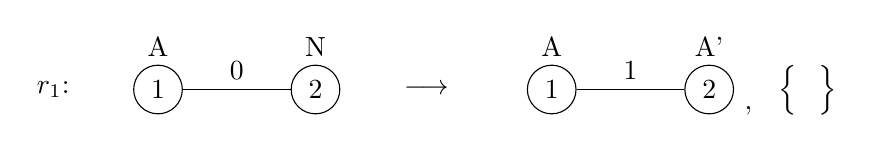
\begin{tikzpicture}
        \draw (-1,0) node[left] {$r_1$:};
        \draw (1,0) node[above] {0};
        
        \node[draw,circle] (x_1) at (0,0) {$1$} ;
        \draw (0,0.3) node[above]{A};
        \node[draw,circle, minimum size = 1pt] (x_2) at (2,0) {$2$};
        \draw (2,0.3) node[above]{N};
        \draw[-] (x_1) -- (x_2);
        
        \draw (3,0) node[right] {$\longrightarrow$};
        \draw (6,0) node[above] {1};
        
        \node[draw,circle] (x3) at (5,0) {$1$} ;
        \draw (5,0.3) node[above]{A};
        \node[draw,circle, minimum size = 1pt] (x4) at (7,0) {$2$};
        \draw (7,0.3) node[above]{A'};
        \draw (7.5,-0.45) node[above]{$,$};
        \draw (8,-0.45) node[above]{$\Big\{$};
        \draw (8.5,-0.45) node[above]{$\Big\}$};
        \draw[-] (x3) -- (x4);
      \end{tikzpicture}
      
      \noindent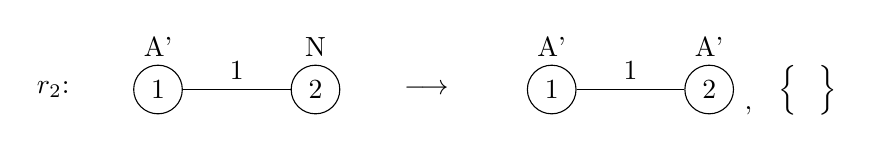
\begin{tikzpicture}
        \draw (-1,0) node[left] {$r_2$:};
        \draw (1,0) node[above] {1};
        
        \node[draw,circle] (x_1) at (0,0) {$1$} ;
        \draw (0,0.3) node[above]{A'};
        \node[draw,circle, minimum size = 1pt] (x_2) at (2,0) {$2$};
        \draw (2,0.3) node[above]{N};
        \draw[-] (x_1) -- (x_2);
        
        \draw (3,0) node[right] {$\longrightarrow$};
        \draw (6,0) node[above] {1};
        
        \node[draw,circle] (x3) at (5,0) {$1$} ;
        \draw (5,0.3) node[above]{A'};
        \node[draw,circle, minimum size = 1pt] (x4) at (7,0) {$2$};
        \draw (7,0.3) node[above]{A'};
        \draw (7.5,-0.45) node[above]{$,$};
        \draw (8,-0.45) node[above]{$\Big\{$};
        \draw (8.5,-0.45) node[above]{$\Big\}$};
        \draw[-] (x3) -- (x4);
      \end{tikzpicture}

      \noindent 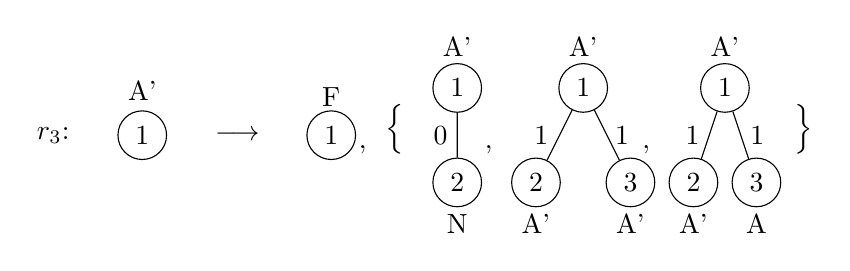
\begin{tikzpicture}[scale = 0.8]
        \draw (-1,0) node[left] {$r_3$:};
        
        \node[draw,circle] (x_1) at (0,0) {$1$} ;
        \draw (0,0.4) node[above]{A'};
        
        \draw (1,0) node[right] {$\longrightarrow$};
        
        \node[draw,circle] (x3) at (3,0) {$1$} ;
        \draw (3,0.3) node[above]{F};
        
        %context 1
        \node[draw,circle](c1_1) at (5,0.75) {$1$};
        \draw (5,1.1) node[above] {A'};
        \node[draw,circle](c1_2) at (5,-0.75){$2$};
        \draw (5,-1.1) node[below] {N};
        \draw (5,0) node[left] {$0$};
        \draw[-] (c1_1)--(c1_2);
        \draw (5.5,-0.45) node[above]{$,$};
        
        %context 2
        \node[draw,circle](c2_1) at (7,0.75) {$1$};
        \draw (7,1.1) node[above] {A'};
        \draw (6.25,-1.1) node[below] {A'};
        \draw (7.75,-1.1) node[below] {A'};
        \node[draw,circle](c2_2) at (6.25,-0.75) {$2$};
        \node[draw,circle](c2_3) at (7.75,-0.75) {$3$};
        \draw[-] (c2_1) -- (c2_2);
        \draw (6.6,0) node[left] {$1$};
        \draw (7.35,0) node[right] {$1$};
        \draw[-] (c2_1) -- (c2_3);
        \draw (8,-0.45) node[above]{$,$};
        
        %context 3
        \node[draw,circle](c3_1) at (9.25, 0.75) {$1$};
        \node[draw,circle](c3_2) at (8.75, -0.75) {$2$};
        \node[draw,circle](c3_3) at (9.75, -0.75) {$3$};
        \draw (9.25,1.1)     node[above] {A'};
        \draw (8.75,-1.1) node[below] {A'};
        \draw (9.75,-1.1) node[below] {A};
        \draw (9,0) node[left] {$1$};
        \draw (9.5,0) node[right] {$1$};
        \draw[-] (c3_1) -- (c3_2);
        \draw[-] (c3_1) -- (c3_3);
        
        
        \draw (3.5,-0.45) node[above]{$,$};
        \draw (4,-0.45) node[above]{$\Big\{$};
        \draw (10.5,-0.45) node[above]{$\Big\}$};
      \end{tikzpicture} 

      %execution
      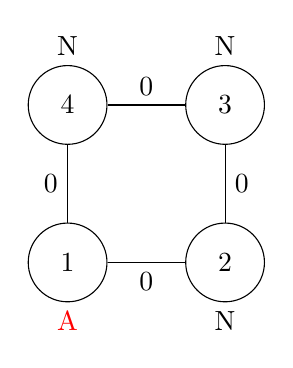
\begin{tikzpicture}
        \node[draw, circle, minimum size = 1 cm] (n1) at (0,0) {$1$};
        \node[draw, circle, minimum size = 1 cm] (n2) at (2,0) {$2$};
        \node[draw, circle, minimum size = 1 cm] (n3) at (2,2) {$3$};
        \node[draw, circle, minimum size = 1 cm] (n4) at (0,2) {$4$};
        
        \draw[-] (n1)--(n2)--(n3)--(n4);
        \draw[-] (n4)--(n1);
        
        \draw(0,-0.5) node[below] {\textcolor{red}{ A}};
        \draw(2,-0.5) node[below] {N};
        \draw(2,2.5) node[above] {N};
        \draw(0,2.5) node[above] {N};
        
        \draw(1,0) node[below] {0};
        \draw(2,1) node[right] {0};
        \draw(1,2) node[above] {0};
        \draw(0,1) node[left] {0};
        
      \end{tikzpicture}
      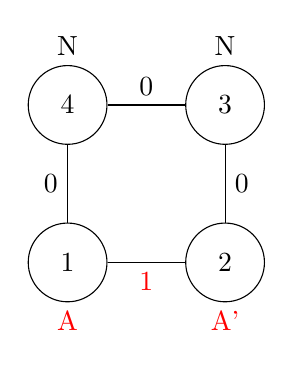
\begin{tikzpicture}
        \node[draw, circle, minimum size = 1 cm] (n1) at (0,0) {$1$};
        \node[draw, circle, minimum size = 1 cm] (n2) at (2,0) {$2$};
        \node[draw, circle, minimum size = 1 cm] (n3) at (2,2) {$3$};
        \node[draw, circle, minimum size = 1 cm] (n4) at (0,2) {$4$};
        
        \draw[-] (n1)--(n2)--(n3)--(n4);
        \draw[-] (n4)--(n1);
        
        \draw(0,-0.5) node[below] {\textcolor{red}{ A}};
        \draw(2,-0.5) node[below] {\textcolor{red}{A'}};
        \draw(2,2.5) node[above] {N};
        \draw(0,2.5) node[above] {N};
        
        \draw(1,0) node[below] {\textcolor{red}{1}};
        \draw(2,1) node[right] {0};
        \draw(1,2) node[above] {0};
        \draw(0,1) node[left] {0};
        
      \end{tikzpicture}
      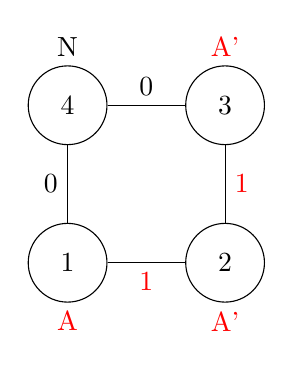
\begin{tikzpicture}
        \node[draw, circle, minimum size = 1 cm] (n1) at (0,0) {$1$};
        \node[draw, circle, minimum size = 1 cm] (n2) at (2,0) {$2$};
        \node[draw, circle, minimum size = 1 cm] (n3) at (2,2) {$3$};
        \node[draw, circle, minimum size = 1 cm] (n4) at (0,2) {$4$};
        
        \draw[-] (n1)--(n2)--(n3)--(n4);
        \draw[-] (n4)--(n1);
        
        \draw(0,-0.5) node[below] {\textcolor{red}{A}};
        \draw(2,-0.5) node[below] {\textcolor{red}{A'}};
        \draw(2,2.5) node[above] {\textcolor{red}{A'}};
        \draw(0,2.5) node[above] {N};
        
        \draw(1,0) node[below] {\textcolor{red}{1}};
        \draw(2,1) node[right] {\textcolor{red}{1}};
        \draw(1,2) node[above] {0};
        \draw(0,1) node[left] {0};
        
      \end{tikzpicture}
      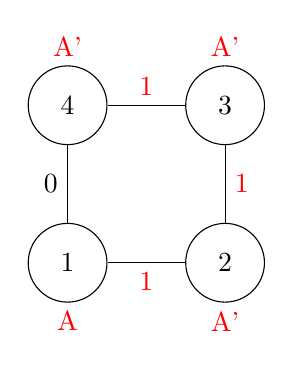
\begin{tikzpicture}
        \node[draw, circle, minimum size = 1 cm] (n1) at (0,0) {$1$};
        \node[draw, circle, minimum size = 1 cm] (n2) at (2,0) {$2$};
        \node[draw, circle, minimum size = 1 cm] (n3) at (2,2) {$3$};
        \node[draw, circle, minimum size = 1 cm] (n4) at (0,2) {$4$};
        
        \draw[-] (n1)--(n2)--(n3)--(n4);
        \draw[-] (n4)--(n1);
        
        \draw(0,-0.5) node[below] {\textcolor{red}{A}};
        \draw(2,-0.5) node[below] {\textcolor{red}{A'}};
        \draw(2,2.5) node[above] {\textcolor{red}{A'}};
        \draw(0,2.5) node[above] {\textcolor{red}{A'}};
        
        \draw(1,0) node[below] {\textcolor{red}{1}};
        \draw(2,1) node[right] {\textcolor{red}{1}};
        \draw(1,2) node[above] {\textcolor{red}{1}};
        \draw(0,1) node[left] {0};
      \end{tikzpicture}
      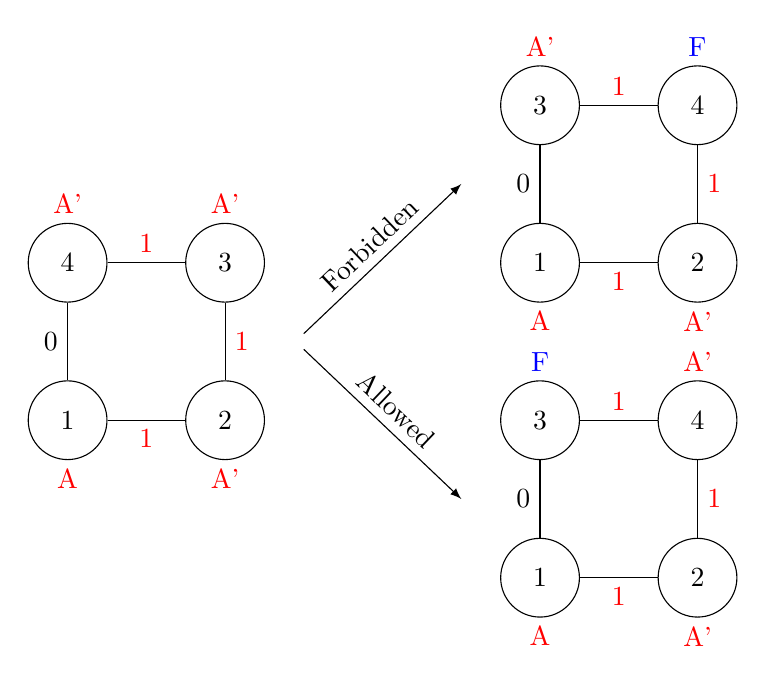
\begin{tikzpicture}
        \node[draw, circle, minimum size = 1 cm] (n1) at (0,0) {$1$};
        \node[draw, circle, minimum size = 1 cm] (n2) at (2,0) {$2$};
        \node[draw, circle, minimum size = 1 cm] (n3) at (2,2) {$3$};
        \node[draw, circle, minimum size = 1 cm] (n4) at (0,2) {$4$};
        
        \draw[-] (n1)--(n2)--(n3)--(n4);
        \draw[-] (n4)--(n1);
        
        \draw(0,-0.5) node[below] {\textcolor{red}{A}};
        \draw(2,-0.5) node[below] {\textcolor{red}{A'}};
        \draw(2,2.5) node[above] {\textcolor{red}{A'}};
        \draw(0,2.5) node[above] {\textcolor{red}{A'}};
        
        \draw(1,0) node[below] {\textcolor{red}{1}};
        \draw(2,1) node[right] {\textcolor{red}{1}};
        \draw(1,2) node[above] {\textcolor{red}{1}};
        \draw(0,1) node[left] {0};
        
        
        %right up
        \node[draw, circle, minimum size = 1 cm] (2n1) at (6,2) {$1$};
        \draw (6,1.5) node[below]{\textcolor{red}{A}};
        \node[draw, circle, minimum size = 1 cm] (2n2) at (8,2) {$2$};
        \draw (8,1.5) node[below]{\textcolor{red}{A'}};
        \node[draw, circle, minimum size = 1 cm] (2n3) at (6,4) {$3$};
        \draw (6,4.5) node[above]{\textcolor{red}{A'}};
        \node[draw, circle, minimum size = 1 cm] (2n4) at (8,4) {$4$};
        \draw (8,4.5) node[above]{\textcolor{blue}{F}};
        
        
        \draw[-] (2n1)-- node[midway,below]{\textcolor{red}{1}}(2n2) -- node[midway,right]{\textcolor{red}{1}} (2n4) -- node[midway,above]{\textcolor{red}{1}} (2n3) --node[midway,left]{0} (2n1);
        
        
        %right down
        \node[draw, circle, minimum size = 1 cm] (2n1) at (6,-2) {$1$};
        \draw (6,-2.5) node[below]{\textcolor{red}{A}};
        \node[draw, circle, minimum size = 1 cm] (2n2) at (8,-2) {$2$};
        \draw (8,-2.5) node[below]{\textcolor{red}{A'}};
        \node[draw, circle, minimum size = 1 cm] (2n3) at (6,0) {$3$};
        \draw (6,0.5) node[above]{\textcolor{blue}{F}};
        \node[draw, circle, minimum size = 1 cm] (2n4) at (8,0) {$4$};
        \draw (8,0.5) node[above]{\textcolor{red}{A'}};
        
        
        \draw[-] (2n1)-- node[midway,below]{\textcolor{red}{1}}(2n2) -- node[midway,right]{\textcolor{red}{1}} (2n4) -- node[midway,above]{\textcolor{red}{1}} (2n3) --node[midway,left]{0} (2n1);
        
        \draw[->, >=latex] (3,1.1) to  node[sloped, midway,above]{Forbidden} (5,3);
        \draw[->, >=latex] (3,0.9) to  node[sloped, midway,above]{Allowed} (5,-1);
      \end{tikzpicture}

      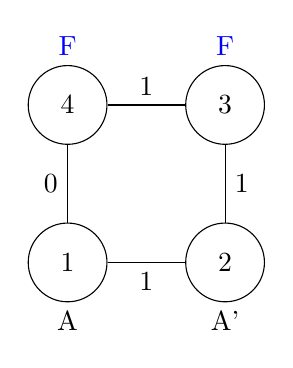
\begin{tikzpicture}
        \node[draw, circle, minimum size = 1 cm] (n1) at (0,0) {$1$};
        \node[draw, circle, minimum size = 1 cm] (n2) at (2,0) {$2$};
        \node[draw, circle, minimum size = 1 cm] (n3) at (2,2) {$3$};
        \node[draw, circle, minimum size = 1 cm] (n4) at (0,2) {$4$};
        
        
        \draw(0,-0.5) node[below] {A};
        \draw(2,-0.5) node[below] {A'};
        \draw(2,2.5) node[above] {\textcolor{blue}{F}};
        \draw(0,2.5) node[above] {\textcolor{blue}{F}};
        
        \draw (n1) --node[midway,below]{1} (n2) -- node[midway,right]{1} (n3) --node[midway,above]{1} (n4) --node[midway,left]{0} (n1);
      
      \end{tikzpicture}

      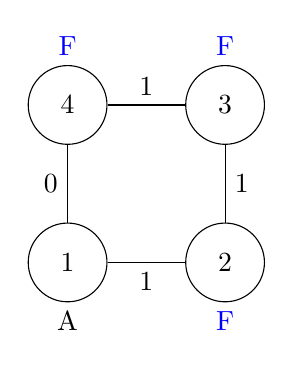
\begin{tikzpicture}
        \node[draw, circle, minimum size = 1 cm] (n1) at (0,0) {$1$};
      \node[draw, circle, minimum size = 1 cm] (n2) at (2,0) {$2$};
      \node[draw, circle, minimum size = 1 cm] (n3) at (2,2) {$3$};
      \node[draw, circle, minimum size = 1 cm] (n4) at (0,2) {$4$};
      
      
      \draw(0,-0.5) node[below] {A};
      \draw(2,-0.5) node[below] {\textcolor{blue}{F}};
      \draw(2,2.5) node[above] {\textcolor{blue}{F}};
      \draw(0,2.5) node[above] {\textcolor{blue}{F}};
      
      \draw (n1) --node[midway,below]{1} (n2) -- node[midway,right]{1} (n3) --node[midway,above]{1} (n4) --node[midway,left]{0} (n1);
        
      \end{tikzpicture}
      \end{example}
      
      % \begin{definition}[FCGLS \cite{litovsky1999graph} ]
      %   \todo[tickmarkheight=0.1cm]{todo}
      % Let $(G,\lambda)$ be a labelled graph. A context of $(G,\lambda)$ is a triple $(H,\mu,\psi)$
      %  such that $(H,\mu)$ is a labelled graph and $\psi$ an occurrence of $(G,\lambda)$ in $(H,\mu)$.
          
      % A relabelling rule with forbidden contexts is a 4-tuple $R=(G_R,\lambda_R,\lambda'_R,F_R)$ such 
      % that $(G_R,\lambda_R,\lambda'_R)$.
          
      % A graph relabelling system with forbidden contexts (FCGRS) is a triple $\mathcal{R} = (L,I,P)$ 
      % defined as a GRS except that the set P is a set of relabelling rules with forbidden contexts. 
      % \end{definition}
      
      
      % \begin{definition}[Graph Relabeling System With priorities and Forbidden Contexts \cite{litovsky1999graph}]
      %   Let $\mathcal{R}$ be a set of graph relabeling rules,  $>$ a strict partial order on $\mathcal{R}$, and $f$ a function associating to every rule $r$ a set of morphisms from $lhs(r)$ in \textbf{Graph}.  For all labeled graph $H$, for all $r\mathcal{R}$, let  
      %   \begin{flalign*}
      %     \f{F}_{fcpgls}(r) \isdef 
      %     \f{F}_{pgls}(r) \cap \f{F}_{fcgls}(r)
      %   \end{flalign*}
      %   The rewriting system $(\textbf{Graph}, \to_\mathcal{R})$, générated by $\mathcal{R}$ and $\f{F}_{fcpgls}$ is called a \textbf{graph relabeling system with priorities and forbidden contexts} (FCPGLS).
      % \end{definition}
       
      % Let $G,G'$ be two graphs. A \textbf{graph homomorphism} consists of two functions $h_0 : G_v \to G_v'$ and $h_1: G_e \to G_e'$ such that 
      % for all $x \in G_e$
      % \begin{itemize}
      %       \item $G'_s( h_1(x)) = h_0(G_s(x))$ 
      %       \item $G'_t( h_1(x)) = h_0(G_t(x))$  
      %       \item $G'_l( h_1(x)) = G_l(x)$   
      % \end{itemize}